\documentclass[12pt,a4paper,table]{article}

\usepackage[margin=1in]{geometry}
\usepackage{multicol}
\usepackage{listings}
\usepackage{graphicx}
\usepackage{hyperref}
\usepackage{caption}
\usepackage{pgfgantt}
\usepackage{natbib}
\usepackage{multirow}
\usepackage{pdflscape}
\usepackage{longtable}

\renewcommand{\baselinestretch}{1.5}
\def\subsubsectionautorefname{subsection}

\newcommand{\code}[1]{\texttt{#1}}

\graphicspath{{img/}}


\begin{document}


    \begin{titlepage}
        \large{University of Westminster}
        \vspace*{\fill}
        \begin{center}
            \Huge{\textsc{Final Year Project}}\\
            \LARGE{LIEBERT server monitoring platform}\\
            \Large{Requirements report}\\[0.7cm]
            \Large{Martin Kukura}\\
            \Large{w1499573}\\[2.0cm]
            \large{December 2016}\\[3cm]
            \large{Supervisor: Girish Lukka}
        \end{center}
        \vspace*{\fill}
        \center{\Large{ECSC697 - Computer Science And Software Engineering Project}}
    \end{titlepage}
    \pagebreak

    \tableofcontents
    \listoffigures

    \pagebreak


    \section{Statement of purpose}
        \subsection{Synopsis}
            With the evolution of computer systems in the recent years, the cost of processing power has been dropping rapidly. This allows everyone from big corporations to ordinary people to possess vast computing resources, be it in the form of a regular computer, Raspberry Pi or a virtual server instance running in the cloud provided by the likes of \textit{Amazon}. Most companies, as well as many tech savvy consumers utilize these resources to run long-lived continuous tasks such as video encoding or data processing. Without proper monitoring tools, large amounts of computing resources can be wasted, as many instances are provisioned with needlessly large amounts of CPU and RAM due to their relatively low cost. Looking at the bigger picture however, under-utilizing, especially cloud resources, becomes a costly nightmare when the operation being supported scales unexpectedly. On the other hand, many instances are over-utilized and would be able to complete their tasks more efficiently if they were properly dimensioned.

            Server monitoring tools evolved from the need to track system performance. They not only allow system administrators to detect over and under-utilized systems, but also monitor system health. Properly setup advanced monitoring system will not only raise an alert when an issue has arised, but also warn of any impending issues (e.g. disk space running out). There are many monitoring systems out there used to fulfil different requirements. From large complex all-in-one solutions such as \textit{Nagios}, through easy to setup tools like \textit{Munin}, to ones that are focused on performance akin to \textit{collectd}.

            \textbf{LIEBERT}'s main goal will be to end up in the last category. There is a vast array of system monitoring tools, however very few of them focus on performance and memory footprint and instead sacrifice these parameters in favour of more features, many of which are, more often than not, unused. \textbf{LIEBERT} will be written from the ground up to offer superior performance and avoid hogging up the system, and will instead sacrifice features if required.

        \subsection{Project scope}\label{sec:scope}
            \textbf{LIEBERT} will be pretty limited in scope, however it will make up for that fact by going more in-depth in its core features. The minimal basic version will deliver a highly performant monitoring solution with minimal resource usage. There will be two parts (applications), one will be the endpoint metric gatherer that will reside on each monitored node, the other one will be a \textit{controller} to which all the endpoint applications will send their data over the network to store the metrics to persistent storage. The core monitored metrics will be CPU, RAM, HDD and network utilisation. The core storage methods will be plaintext and RRD (round-robin database). \textit{LIEBERT}'s focus is on performant metric retrieval, therefore there will not be any sort of dashboard with fancy charts to display the data. One of the core storage options, RRD, is however designed for easy storage and visualization of timeseries data, and it will therefore be very easy to create visualizations without the need for external software (except for \textit{RRDtool} itself). RRD is also widely used in the industry to store this sort of data, and will therefore be familiar to most people dealing with \textbf{LIEBERT} \citep{rrdtool}. If time restrictions allow for further development after the initial version is finished, there are numerous extra features that can be added, most notably a plugin system that will allow for collection of any user-supplied metric. Note however that the performance of the plugin system would be considerably lower than what core \textbf{LIEBERT} will be able to offer. The initial version of the package will aim for compatibility with the Linux operating system, because it is the most widely used server operating system \citep{systempop}\footnote{Non-public facing server OS market share is impossible to determine, however from personal experience and blogs of leading technology companies Linux seems to be the most popular}.

        \subsection{Goals}
            The primary goal of this project is a learning experience. Creating \textbf{LIEBERT} will require good understanding of all the possible programming languages that could be used to ensure its performance, as well as proper understanding of the chosen programming language to ensure best practices leading to higher performance. It will also require deeper understanding of the targeted operating systems (basic version being aimed at Linux) to minimize resource requirements for the metric gathering itself, as well as networking to enable cross-application communication through the network.
            
            Secondary goal is delivery of the actual monitoring system, with all of the basic, and potentially some of the extra, features described. Altough the software package itself will be a proof-of-concept, maximum care will be taken to deliver as production-ready product as possible.

        \subsection{Stakeholders}
            Due to the relatively closed and autonomous nature of the system, there aren't many direct stakeholders. However, indirectly the system can affect a broad range of entities, as the operation of a monitoring suite and thus healthy state of the underlying system (or rather an unhealthy state of the underlying system) will affect any user consuming services running on top of it. The system will therefore have 2 major stakeholders - the system administrators directly interacting with our monitoring solution, and consumers that depend on the system that is being monitored.
    \section{Context diagram}
        \begin{figure}[!htb]
            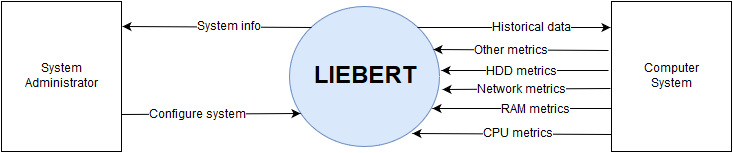
\includegraphics[width=\textwidth]{diagram-context.png}
            \caption{The context diagram}
            \label{fig:diagram-context}
        \end{figure}

        The context diagram provided in \autoref{fig:diagram-context} displays the information flow to and from the system. As said before, the autonomous nature of our system limits its reach, therefore information will only be exchanged with the computer systems that are running the application, and with potential system administrators that are either engaging in maintenance tasks or are checking on the status of the application itself. This type of diagram is also known as the \textit{Data Flow Diagram}.

    \section{Requirements}
        \subsection{Similar software}
            To better understand the requirements for system monitoring software, a survey of some of the most popular existing solutions was performed. Exploring their features and prominent characteristics allowed for a more precise specification on what shall be the focus of this project.

            \subsubsection{Nagios}
                \textit{Nagios} (\url{https://www.nagios.org/}), '\textit{the industry standard in IT infrastructure monitoring}' as it proclaims itself, is an extremely extensible monitoring solution. It doesn't come with any actual data gathering capabilities out of the box, however its plugin architecture allows users to write extensions to monitor anything from system metrics to complex applications. Nagios offers excellent alerting and early warning capabilities atop the user supplied data as well as logging, however its configuration is rather complex. It also comes with a basic but very powerful web dashboard allowing control over the software. The storage backend of \textit{Nagios} is handled by \textit{RRDtool}.
            \subsubsection{Munin}
                \textit{Munin} (\url{http://munin-monitoring.org/}) is an alerting solution similar to \textit{Nagios}, however its main focus is on ease of use. It provides near plug-and-play capabilities and simple configuration and plugin creation. \textit{Munin} uses a master - nodes architecture where
                the master node polls all child nodes for data. Plugins can be written in any language and only require that they be executable and their text output matches \textit{Munin} specifications. It also offers a simple web interface, and stores it's data using \textit{RRDtool}.
            \subsubsection{collectd}
                \textit{Collectd} (\url{https://collectd.org/}) is a minimal filtering and relaying Unix daemon with extensible architecture. Core of \textit{collectd} only provides high performance 'routing' capabilities between various input and output plugins. By default it ships with plugins for collecting cpu, network, load and memory data, as well as output plugins for CSV, RRD, and network relaying. \textit{Collectd} plugins have to be written in C and are loaded as shared modules - this makes them highly efficient and performant, however makes them incredibly difficult to make for someone who is not well-versed in C.

            \subsubsection{Feature table}
                To better understand the differences between the aforementioned monitoring solutions, a feature comparison table has been created. It shows clear difference between the features, and allows cherry-picking characteristics of each solution that should be part of \textbf{LIEBERT}.

                \begin{center}
                    \begin{tabular}{ |c|c|c|c|c| }
                        \hline
                            Features & \textbf{Nagios} & \textbf{Munin} & \textbf{collectd} & \textbf{LIEBERT}\\
                            \hline
                            \textbf{Extensible} & Yes & Yes & Yes & Extra feature\\
                            \hline
                            \textbf{Easy to extend} & No & Yes & No & Extra feature - Yes\\
                            \hline
                            \textbf{Core monitoring included} & No & Yes & Yes & Yes\\
                            \hline
                            \textbf{Web dashboard} & Yes & Yes & No & No\\
                            \hline
                            \textbf{Easy to use} & No & Yes & No & Yes\\
                            \hline
                            \textbf{Focused on performance} & No & No & Yes & Yes\\
                            \hline
                            \textbf{Cross-platform} & No & No & No & Partially\\
                        \hline
                    \end{tabular}
                \end{center}

                \paragraph{Extensibility}
                    Extensibility is not planned as an essential part of \textbf{LIEBERT}. This is due to the fact that important metric collectors will be included as part of the system core, and therefore optimized. Extensibility, if implemented will be working on the same principle as \textit{Munin}, where \textbf{LIEBERT} will call user supplied executables that will provide data in specific format recognizable by the system.

                \paragraph{Web dashboard}
                    The aim of this project is to create a highly performant system with minimal memory footprint. In order to achieve that, certain features need to be sacrificed. Web accessibility (and advanced user interaction in general) is not included in the project as such features would most probably be more resource intensive than \textbf{LIEBERT} itself.

                \paragraph{Easy to use}
                    Ease of use is probably the second most important requirement after performance. This will enable users to make use of high performance monitoring without the steep learning curve of tools such as \textit{collectd}. \textbf{LIEBERT} will strive to provide an easy setup and configuration akin to \textit{Munin}, where users should be able to get basic monitoring started just by changing a few lines in a configuration file.

                \paragraph{Performance}
                    Primary requirement of this project is performance. Features will be sacrificed to provide high performance and small memory footprint (compared to other full-featured solutions). The system will be implemented in a low level language to ensure no performance overhead arising from complex modern languages.

                \paragraph{Cross-platform}
                    Altough \textbf{LIEBERT} will not be intentionally developed for cross-platform compatibility, it will be very easy to port to other platforms due to the chosen programming language (read more in \autoref{sec:language}). In fact, most of it will be written in cross-platform compatible code and the only parts that will need rewriting are the gatherer modules which utilize native OS resources.

        \subsection{Programming language}\label{sec:language}
            In order to maximize performance of the system, care needs to be taken when choosing the language it will be implemented in. Choice of an unsuitable language might effectively 'undo' any optimizations done within the code, as the language's execution environment can be a source of large resource utilization. This is especially true for hybrid \textit{JIT} compiled languages such as Java or C\#. In the following subsections the results of surveying for potentially suitable languages can be found.

            \subsubsection{C / C++}
                \textit{C}, or "The closest you can get to assembler"\footnote{Quote from an old coworker}, is a low-level, immensly powerful and versatile language with practically zero overhead. It enables programmers to create highly optimized applications, however its 'freedom' can (and will) lead to negative side-effects such as no memory safety. \textit{C++} is an evolution of \textit{C} that added modern features on top of the old language, such as objects. These two languages would be suitable for the project, however their inherent memory unsafety can be a problem.

            \subsubsection{Go}
                \textit{Go} is a modern systems programming language created by \textit{Google}. It has seen surge of popularity since its public release in 2009, especially in recent years. It offers similar low-level system access as the \textit{C} family, however was designed for concurrent applications and therefore contains built-in concurrency and memory safety features. It also features a garbage collector found in many modern high-level languages. \textit{Go} would be a fantastic fit for \textbf{LIEBERT}, however its use of the garbage collector is a downside.

            \subsubsection{Rust}
                \textit{Mozilla}'s very own programming language \textit{Rust}, publicly announced in 2010, has seen recent surge in popularity in the same way as \textit{Go}. Rust is essentially a very low-level language akin to \textit{C}, without any additional overhead of a garbage collector that \textit{Go} has. It is also focused on concurrency and memory safety, and additionally contains so called \textit{zero-cost abstractions}. \textit{Zero-cost abstractions} are compile-time features that allow the language to have powerful features often found in higher level languages, however with practically zero overhead. This is accomplished by the \textit{Rust} compiler that performs complicated analysis and optimization, that's additionally able to perform actions such as unrolling highly complex loops \citep{asseldonk}. Notable features of the language is the lack of objects, native support for creating and distributing libraries, memory safety (mostly accomplished by the so called \textit{borrow checker}), type inference, and its focus on concurrency.

            \subsubsection{Python}
                \textit{Python} is the most popular interpreted programming language \citep{tiobe}. Years of development surprisingly allowed it to mature into a powerful and incredibly fast interpreter. It doesn't have a set goal or focus in mind, and is instead a general programming language capable of producing nearly any sort of application. \textit{Python} provides convenience features found in many high-level programming languages, such as dynamic typing or a garbage collector. Altough it is considerably fast, it's still going to suffer from overhead compared to low-level compiled programming languages.

            \subsubsection{Feature table}
                \begin{center}
                    \begin{tabular}{ |c|c|c|c|c|c| }
                        \hline
                            Features & \textbf{C / C++} & \textbf{Go} & \textbf{Rust} & \textbf{Python} & \textbf{Desired?}\\
                            \hline
                            \textbf{Low-level} & Yes & Yes & Yes & No & Yes\\
                            \hline
                            \textbf{Garbage collector} & No & Yes & No & Yes & No\\
                            \hline
                            \textbf{Dynamic typing} & No & No & No & Yes & No\\
                            \hline
                            \textbf{Conveniece features} & No & Somewhat & Yes & Yes & Yes\\
                            \hline
                            \textbf{Runtime overhead} & No & Small & No & Large & No\\
                            \hline
                            \textbf{Cross-platform} & Yes & Yes & Yes & Yes & Yes\\
                            \hline
                            \textbf{Memory safety} & No & Yes & Yes & Partially & Yes\\
                        \hline
                    \end{tabular}
                \end{center}

            \subsubsection{Conclusion}
                \paragraph{Programming language}
                    The implementation language chosen for this project is \textbf{Rust}. It features many high-level language convenience features through its \textit{zero-cost abstraction} system, focuses on concurrency, and does not come with any added overhead of the likes of a garbage collector.

                \paragraph{Development methodology}
                    Traditional methodologies such as \textit{waterfall} are becoming less and less popular in modern software development. Altough still present, they are often remnants of the old times in large corporations with established workflows. Evolving progressive teams and new companies alike are usually not in favour of such methodologies, and instead prefer modern ones such as \textit{Agile} to enable rapid feature development, leveraging continuos integration and deployment to push new releases into production as quickly as possible. This project will embrace the \textit{agile-scrum} methodology, focusing on design, development and release of features in small batches. This is relevant to the Gantt chart found in \autoref{sec:gantt}, which indicates a longer running design and development cycle in the first phase of the project that focuses on delivering a minimal working version, with short-release feature development cycles in the second phase.

        \subsection{Functional requirements}
            The system will consist of 2 applications, an \textit{Agent} and a \textit{Controller}. Each has its own set of requirements.

            \subsubsection{Agent}
                \begin{tabular}{ p{0.7cm}|p{14.5cm} }
                    \multirow{3}{*}{R1 } & \textbf{The application shall collect CPU state metrics}\\
                    \cline{2-2}
                    & The application should extract CPU load counters from the underlying operating system with as much granularity as possible. These should at least include user and system load.\\
                    \cline{2-2}
                    & Importance: \textbf{essential}
                \end{tabular}

                \vspace{0.5cm}
                \noindent
                \begin{tabular}{ p{0.7cm}|p{14.5cm} }
                    \multirow{3}{*}{R2 } & \textbf{The application shall collect RAM state metrics}\\
                    \cline{2-2}
                    & The application should extract current RAM usage from the underlying operating system. This should include utilized RAM as a minimum.\\
                    \cline{2-2}
                    & Importance: \textbf{essential}
                \end{tabular}

                \vspace{0.5cm}
                \noindent
                \begin{tabular}{ p{0.7cm}|p{14.5cm} }
                    \multirow{3}{*}{R3 } & \textbf{The application shall collect HDD state metrics}\\
                    \cline{2-2}
                    & The application should extract current disk usage from the underlying operating system. This should include the primary partition as a minimum.\\
                    \cline{2-2}
                    & Importance: \textbf{essential}
                \end{tabular}

                \vspace{0.5cm}
                \noindent
                \begin{tabular}{ p{0.7cm}|p{14.5cm} }
                    \multirow{3}{*}{R4 } & \textbf{The application shall collect network interface metrics}\\
                    \cline{2-2}
                    & The application should extract network throughput and interface information from the underlying operating system.\\
                    \cline{2-2}
                    & Importance: \textbf{essential}
                \end{tabular}

                \vspace{0.5cm}
                \noindent
                \begin{tabular}{ p{0.7cm}|p{14.5cm} }
                    \multirow{3}{*}{R5 } & \textbf{The application shall store collected data in an internal buffer}\\
                    \cline{2-2}
                    & The application should accumulate gathered metrics in an internal structure until they are ready to be sent over the network to the connected \textit{Controller} instance.\\
                    \cline{2-2}
                    & Importance: \textbf{essential}
                \end{tabular}

                \vspace{0.5cm}
                \noindent
                \begin{tabular}{ p{0.7cm}|p{14.5cm} }
                    \multirow{3}{*}{R6 } & \textbf{The application shall connect to a controller instance}\\
                    \cline{2-2}
                    & The application should establish a TCP link with a relevant controller on the network. This connection will be used to forward metric data and receive control commands.\\
                    \cline{2-2}
                    & Importance: \textbf{desired}
                \end{tabular}

                \vspace{0.5cm}
                \noindent
                \begin{tabular}{ p{0.7cm}|p{14.5cm} }
                    \multirow{3}{*}{R7 } & \textbf{The application shall forward the stored data to a connected Controller instance}\\
                    \cline{2-2}
                    & The application should periodically forward accumulated metric data to a connected \textit{Controller} instance. In case the \textit{Controller} is unavailable, it should keep accumulating data internally until the \textit{Controller} becomes available.\\
                    \cline{2-2}
                    & Importance: \textbf{desired}
                \end{tabular}

                \vspace{0.5cm}
                \noindent
                \begin{tabular}{ p{0.7cm}|p{14.5cm} }
                    \multirow{3}{*}{R8 } & \textbf{The application shall be extendable}\\
                    \cline{2-2}
                    & Users should be able to extend the gathering capabilities with custom executables providing output recognizable by the system.\\
                    \cline{2-2}
                    & Importance: \textbf{luxury}
                \end{tabular}

                \vspace{0.5cm}
                \noindent
                \begin{tabular}{ p{0.7cm}|p{14.5cm} }
                    \multirow{3}{*}{R9 } & \textbf{The user shall be able to configure all parts of the application}\\
                    \cline{2-2}
                    & The application should be configurable in all areas where it makes sense. This would include network, gathering, and storage configuration at minimum.\\
                    \cline{2-2}
                    & Importance: \textbf{desirable}
                \end{tabular}

                \vspace{0.5cm}
                \noindent
                \begin{tabular}{ p{0.7cm}|p{14.5cm} }
                    \multirow{3}{*}{R10} & \textbf{The application shall log important runtime information}\\
                    \cline{2-2}
                    & The application should print \textit{debug} / \textit{warning} / \textit{info} messages either to to \textit{stdout} or a file.\\
                    \cline{2-2}
                    & Importance: \textbf{essential}
                \end{tabular}

                \vspace{0.5cm}
                \noindent
                \begin{tabular}{ p{0.7cm}|p{14.5cm} }
                    \multirow{3}{*}{R11} & \textbf{The user shall be able to check the application's current status}\\
                    \cline{2-2}
                    & There should be a way to 'tap into' the application and review its current status. This should probably be implemented as an additional protocol over the network.\\
                    \cline{2-2}
                    & Importance: \textbf{luxury}
                \end{tabular}


            \subsubsection{Controller}
                \begin{tabular}{ p{0.7cm}|p{14.5cm} }
                    \multirow{3}{*}{R12} & \textbf{The application shall receive connections from \textit{Agents}}\\
                    \cline{2-2}
                    & The application should be able to establish TCP connections with \textit{Agents} on the network.\\
                    \cline{2-2}
                    & Importance: \textbf{essential}
                \end{tabular}

                \vspace{0.5cm}
                \noindent
                \begin{tabular}{ p{0.7cm}|p{14.5cm} }
                    \multirow{3}{*}{R13} & \textbf{The application shall authenticate connecting \textit{Agents}}\\
                    \cline{2-2}
                    & The application should implement security protocols to only allow connections from authorized \textit{Agents}.\\
                    \cline{2-2}
                    & Importance: \textbf{luxury}
                \end{tabular}

                \vspace{0.5cm}
                \noindent
                \begin{tabular}{ p{0.7cm}|p{14.5cm} }
                    \multirow{3}{*}{R14} & \textbf{The application shall receive data from connected \textit{Agents}}\\
                    \cline{2-2}
                    & The application should be able to handle historical metric data received from all connected \textit{Agents}\\
                    \cline{2-2}
                    & Importance: \textbf{essential}
                \end{tabular}

                \vspace{0.5cm}
                \noindent
                \begin{tabular}{ p{0.7cm}|p{14.5cm} }
                    \multirow{3}{*}{R15} & \textbf{The application shall store data into persistent storage}\\
                    \cline{2-2}
                    & The application should store the historical metric data received from \textit{Agents} to persistent storage (e.g. hard drive) in one of the supported formats.\\
                    \cline{2-2}
                    & Importance: \textbf{essential}
                \end{tabular}

                \vspace{0.5cm}
                \noindent
                \begin{tabular}{ p{0.7cm}|p{14.5cm} }
                    \multirow{3}{*}{R16} & \textbf{The application shall store data using plaintext format}\\
                    \cline{2-2}
                    & The application should be able to store data to persistent storage using a suitable plaintext format.\\
                    \cline{2-2}
                    & Importance: \textbf{essential}
                \end{tabular}

                \vspace{0.5cm}
                \noindent
                \begin{tabular}{ p{0.7cm}|p{14.5cm} }
                    \multirow{3}{*}{R17} & \textbf{The application shall store data using \textit{RRD} format}\\
                    \cline{2-2}
                    & The application should be able to store data to persistent storage using the format supported by \textit{RRDtool}.\\
                    \cline{2-2}
                    & Importance: \textbf{desired}
                \end{tabular}

                \vspace{0.5cm}
                \noindent
                \begin{tabular}{ p{0.7cm}|p{14.5cm} }
                    \multirow{3}{*}{R18} & \textbf{The application shall store data into a database}\\
                    \cline{2-2}
                    & The application should be able to store data into a relational database such as \textit{SQLite} or \textit{MySQL}.\\
                    \cline{2-2}
                    & Importance: \textbf{luxury}
                \end{tabular}

                \vspace{0.5cm}
                \noindent
                \begin{tabular}{ p{0.7cm}|p{14.5cm} }
                    \multirow{3}{*}{R19} & \textbf{The application shall be extendable}\\
                    \cline{2-2}
                    & The output formats of the application should be extendable using user supplied executables that accept a predefined format of the system.\\
                    \cline{2-2}
                    & Importance: \textbf{luxury}
                \end{tabular}

                \vspace{0.5cm}
                \noindent
                \begin{tabular}{ p{0.7cm}|p{14.5cm} }
                    \multirow{3}{*}{R20} & \textbf{The user shall be able to configure all parts of the application}\\
                    \cline{2-2}
                    & The application should be configurable in all areas where it makes sense. This would include network and storage configuration at minimum.\\
                    \cline{2-2}
                    & Importance: \textbf{desired}
                \end{tabular}

                \vspace{0.5cm}
                \noindent
                \begin{tabular}{ p{0.7cm}|p{14.5cm} }
                    \multirow{3}{*}{R21} & \textbf{The user shall be able to check the application's current status}\\
                    \cline{2-2}
                    & There should be a way to 'tap into' the application and review its current status. This should probably be implemented as an additional protocol over the network.\\
                    \cline{2-2}
                    & Importance: \textbf{luxury}
                \end{tabular}

                \vspace{0.5cm}
                \noindent
                \begin{tabular}{ p{0.7cm}|p{14.5cm} }
                    \multirow{3}{*}{R22} & \textbf{The user shall be able to relay commands to all connected \textit{Agents}}\\
                    \cline{2-2}
                    & The user should be able to utilize the \textit{Controller's} connections to relay commands to connected \textit{Agent} instances. This requirement is closely related to '\textit{The user shall be able to check the application's current status}'.\\
                    \cline{2-2}
                    & Importance: \textbf{luxury}
                \end{tabular}

                \vspace{0.5cm}
                \noindent
                \begin{tabular}{ p{0.7cm}|p{14.5cm} }
                    \multirow{3}{*}{R23} & \textbf{The application shall log important runtime information}\\
                    \cline{2-2}
                    & The application should print \textit{debug} / \textit{warning} / \textit{info} messages either to to \textit{stdout} or a file.\\
                    \cline{2-2}
                    & Importance: \textbf{essential}
                \end{tabular}



        \subsection{Non-functional requirements}
            \begin{tabular}{ p{0.7cm}|p{14.5cm} }
                \multirow{3}{*}{NF1} & \textbf{The system shall be built with focus on performance}\\
                \cline{2-2}
                & Maximum care should be taken when designing and developing the project to ensure maximum performance of the end result.\\
                \cline{2-2}
                & Importance: \textbf{essential}
            \end{tabular}

            \vspace{0.5cm}
            \noindent
            \begin{tabular}{ p{0.7cm}|p{14.5cm} }
                \multirow{3}{*}{NF2} & \textbf{The system shall be written in the \textit{Rust} programming language}\\
                \cline{2-2}
                & After careful consideration of multiple programming languages (discussed in \autoref{sec:language}) the \textit{Rust} programming language has been chosen due to its best feature-to-performance ratio.\\
                \cline{2-2}
                & Importance: \textbf{essential}
            \end{tabular}

            \vspace{0.5cm}
            \noindent
            \begin{tabular}{ p{0.7cm}|p{14.5cm} }
                \multirow{3}{*}{NF3} & \textbf{The system shall target the Linux operating system}\\
                \cline{2-2}
                & As discussed in \autoref{sec:scope}, primary support for Linux has been chosen due to its popularity with servers.\\
                \cline{2-2}
                & Importance: \textbf{essential}
            \end{tabular}

            \vspace{0.5cm}
            \noindent
            \begin{tabular}{ p{0.7cm}|p{14.5cm} }
                \multirow{3}{*}{NF4} & \textbf{The various system parts shall communicate through a network}\\
                \cline{2-2}
                & Due to the nature of \textit{Agent} and \textit{Controller}, network communication will be required to utilize all the features of the system.\\
                \cline{2-2}
                & Importance: \textbf{essential}
            \end{tabular}

            \vspace{0.5cm}
            \noindent
            \begin{tabular}{ p{0.7cm}|p{14.5cm} }
                \multirow{3}{*}{NF5} & \textbf{The system shall be built with focus on ease of use}\\
                \cline{2-2}
                & The system should be as easy to use as possible, ideally being able to be utilized with only a few changed lines in a configuration file.\\
                \cline{2-2}
                & Importance: \textbf{essential}
            \end{tabular}

            \vspace{0.5cm}
            \noindent
            \begin{tabular}{ p{0.7cm}|p{14.5cm} }
                \multirow{3}{*}{NF6} & \textbf{The system shall be secure}\\
                \cline{2-2}
                & The system should make use of good modern security practices to not open the network it's residing on to unauthorized entities and prevent tampering with its data.\\
                \cline{2-2}
                & Importance: \textbf{luxury}
            \end{tabular}

            \vspace{0.5cm}
            \noindent
            \begin{tabular}{ p{0.7cm}|p{14.5cm} }
                \multirow{3}{*}{NF7} & \textbf{The system shall have minimal memory footprint}\\
                \cline{2-2}
                & Due to the system's focus on performance, it should also consume minimum resource on the system it is running on.\\
                \cline{2-2}
                & Importance: \textbf{essential}
            \end{tabular}

            \vspace{0.5cm}
            \noindent
            \begin{tabular}{ p{0.7cm}|p{14.5cm} }
                \multirow{3}{*}{NF8} & \textbf{The system's data shall be accurate}\\
                \cline{2-2}
                & Maximum care should be taken to ensure the data retrieved by the system accurately represents the real state.\\
                \cline{2-2}
                & Importance: \textbf{essential}
            \end{tabular}

    \pagebreak

    \section{Use cases}
        Closed and autonomous nature of the system makes regular use case modelling rather hard, however use case modelling still remains important to uncover the various flows within an application. Therefore, instead of focusing on traditional user-oriented use cases, this section will also contain internal system flows such as metric gathering or network communication.

        \subsection{Use case diagram}
            \begin{center}
                \begin{figure}[!h]
                    \includegraphics[width=\textwidth]{diagram-usecase.png}
                    \caption{The use case diagram}
                    \label{fig:diagram-usecase}
                \end{figure}
            \end{center}

        \pagebreak

        \subsection{Use case specifications}
            \begin{longtable}{ |c|p{11.8cm}| }
                \hline
                \multicolumn{2}{|c|}{\cellcolor{lime} \textbf{UC\_1}}\\ \hline
                \cellcolor[gray]{0.9} \textbf{Use case} & Start \textit{Agent}\\ \hline
                \cellcolor[gray]{0.9} \textbf{Description} & Administrator attempts to start the \textit{Agent} application using the operating system's appropriate method\\ \hline
                \cellcolor[gray]{0.9} \textbf{Actors} & Administrator, \textit{Agent}\\ \hline
                \cellcolor[gray]{0.9} \textbf{Pre-conditions} & Application is present on target machine and target machine is running a supported platform\\ \hline
                \multicolumn{2}{|c|}{\cellcolor[gray]{0.9} \textbf{Flow of events}}\\ \hline
                \multicolumn{2}{|l|}{\cellcolor[gray]{0.9} \textbf{Normal flow}}\\ \hline
                \multicolumn{2}{|p{14cm}|}{
                    \begin{enumerate}
                        \item Administrator launches application
                        \item Application parses command line options
                        \item Application loads and parses relevant configuration file
                        \item Application attempts to connect to a configured controller
                        \item Application starts all metric gathering subsystems
                        \item Application enters normal run loop
                    \end{enumerate}
                }\\ \hline
                \multicolumn{2}{|l|}{\cellcolor[gray]{0.9} \textbf{Alternative flow}}\\ \hline
                \multicolumn{2}{|p{14cm}|}{
                    \begin{itemize}
                        \item N/A
                    \end{itemize}
                }\\ \hline
                \cellcolor[gray]{0.9} \textbf{Exceptions} &
                    \begin{itemize}
                        \item If in step 3 the application cannot find a relevant configuration file it exits with an error
                        \item If in step 3 the application cannot successfuly parse the configuration file it exits with an error
                        \item If maximum retries are exceeded in step 4 the application exits with an error
                        \item If a subsystem fails to load in step 5, the application moves it to disabled state and continues
                    \end{itemize}\\ \hline
                \cellcolor[gray]{0.9} \textbf{Post-conditions} & The application is successfuly started and running\\ \hline
            \end{longtable}

            \vspace{0.5cm}
            \noindent
            \begin{longtable}{ |c|p{11.8cm}| }
                \hline
                \multicolumn{2}{|c|}{\cellcolor{lime} \textbf{UC\_2}}\\ \hline
                \cellcolor[gray]{0.9} \textbf{Use case} & Start \textit{Controller}\\ \hline
                \cellcolor[gray]{0.9} \textbf{Description} & Administrator attempts to start the \textit{Controller} application using the operating system's appropriate method\\ \hline
                \cellcolor[gray]{0.9} \textbf{Actors} & Administrator, \textit{Controller}\\ \hline
                \cellcolor[gray]{0.9} \textbf{Pre-conditions} & Application is present on target machine and target machine is running a supported platform\\ \hline
                \multicolumn{2}{|c|}{\cellcolor[gray]{0.9} \textbf{Flow of events}}\\ \hline
                \multicolumn{2}{|l|}{\cellcolor[gray]{0.9} \textbf{Normal flow}}\\ \hline
                \multicolumn{2}{|p{14cm}|}{
                    \begin{enumerate}
                        \item Administrator launches application
                        \item Application parses command line options
                        \item Application loads and parses relevant configuration file
                        \item Application starts all configured storage subsystems
                        \item Application starts listening for \textit{Agent} connections
                        \item Application starts listening for control connections
                        \item Application enters normal run loop
                    \end{enumerate}
                }\\ \hline
                \multicolumn{2}{|l|}{\cellcolor[gray]{0.9} \textbf{Alternative flow}}\\ \hline
                \multicolumn{2}{|p{14cm}|}{
                    \begin{itemize}
                        \item N/A
                    \end{itemize}
                }\\ \hline
                \cellcolor[gray]{0.9} \textbf{Exceptions} & 
                    \begin{itemize}
                        \item If in step 3 the application cannot find a relevant configuration file it exits with an error
                        \item If in step 3 the application cannot successfuly parse the configuration file it exits with an error
                        \item If a subsystem fails to load in step 4, the application moves it to disabled state and continues; if all subsystems fail to load, the application exits with an error
                        \item If the application fails to initialize a TCP listener in step 5 or 6, it exits with an error
                    \end{itemize}\\ \hline
                \cellcolor[gray]{0.9} \textbf{Post-conditions} & The application is successfuly started and running\\ \hline
            \end{longtable}

            \vspace{0.5cm}
            \noindent
            \begin{longtable}{ |c|p{11.8cm}| }
                \hline
                \multicolumn{2}{|c|}{\cellcolor{lime} \textbf{UC\_3}}\\ \hline
                \cellcolor[gray]{0.9} \textbf{Use case} & Configure \textit{Agent}\\ \hline
                \cellcolor[gray]{0.9} \textbf{Description} & The administrator attempts to configure the \textit{Agent} application\\ \hline
                \cellcolor[gray]{0.9} \textbf{Actors} & Administrator, \textit{Agent}, \textit{Controller}\\ \hline
                \cellcolor[gray]{0.9} \textbf{Pre-conditions} & The \textit{Agent} application has been successfuly started; the \textit{Controller} application has been successfuly started and is connected to the relevant \textit{Agent} instance (for alternative flow)\\ \hline
                \multicolumn{2}{|c|}{\cellcolor[gray]{0.9} \textbf{Flow of events}}\\ \hline
                \multicolumn{2}{|l|}{\cellcolor[gray]{0.9} \textbf{Normal flow}}\\ \hline
                \multicolumn{2}{|p{14cm}|}{
                    \begin{enumerate}
                        \item Administrator opens an existing or creates a new configuration file
                        \item Administrator edits the configuration file
                        \item Administrator stops the \textit{Agent} application (if running)
                        \item Administrator starts the \textit{Agent} application - continues in \textbf{UC\_1}
                    \end{enumerate}
                }\\ \hline
                \multicolumn{2}{|l|}{\cellcolor[gray]{0.9} \textbf{Alternative flow}}\\ \hline
                \multicolumn{2}{|p{14cm}|}{
                    \begin{enumerate}
                        \item Administrator successfuly completes \textbf{UC\_5}
                        \item Administrator sends configuration command to \textit{Controller}
                        \item \textit{Controller} relays configuration command to the relevant \textit{Agent}
                        \item \textit{Agent} performs a run-time reconfiguration based on the command received
                    \end{enumerate}
                }\\ \hline
                \cellcolor[gray]{0.9} \textbf{Exceptions} & 
                    \begin{itemize}
                        \item If the command received by \textit{Agent} in \textit{Alternative flow step 3} is invalid, it is discarded and a warning is emitted 
                    \end{itemize}\\ \hline
                \cellcolor[gray]{0.9} \textbf{Post-conditions} & The \textit{Agent} application is successfuly running with the new configuration\\ \hline
            \end{longtable}

            \vspace{0.5cm}
            \noindent
            \begin{longtable}{ |c|p{11.8cm}| }
                \hline
                \multicolumn{2}{|c|}{\cellcolor{lime} \textbf{UC\_4}}\\ \hline
                \cellcolor[gray]{0.9} \textbf{Use case} & Configure \textit{Controller}\\ \hline
                \cellcolor[gray]{0.9} \textbf{Description} & The administrator attempts to configure the \textit{Controller} application\\ \hline
                \cellcolor[gray]{0.9} \textbf{Actors} & Administrator, \textit{Controller}\\ \hline
                \cellcolor[gray]{0.9} \textbf{Pre-conditions} & The \textit{Controller} application has been successfuly started\\ \hline
                \multicolumn{2}{|c|}{\cellcolor[gray]{0.9} \textbf{Flow of events}}\\ \hline
                \multicolumn{2}{|l|}{\cellcolor[gray]{0.9} \textbf{Normal flow}}\\ \hline
                \multicolumn{2}{|p{14cm}|}{
                    \begin{enumerate}
                        \item Administrator opens an existing or creates a new configuration file
                        \item Administrator edits the configuration file
                        \item Administrator stops the \textit{Controller} application (if running)
                        \item Administrator starts the \textit{Controller} application - continues in \textbf{UC\_2}
                    \end{enumerate}
                }\\ \hline
                \multicolumn{2}{|l|}{\cellcolor[gray]{0.9} \textbf{Alternative flow}}\\ \hline
                \multicolumn{2}{|p{14cm}|}{
                    \begin{enumerate}
                        \item Administrator successfuly completes \textbf{UC\_5}
                        \item Administrator sends configuration command to \textit{Controller}
                        \item \textit{Controller} performs run-time reconfiguration based on the command received
                    \end{enumerate}
                }\\ \hline
                \cellcolor[gray]{0.9} \textbf{Exceptions} & 
                    \begin{itemize}
                        \item If the command received by the \textit{Controller} in \textit{Alternative flow step 2} is invalid, it is discarded and a warning is emitted
                    \end{itemize}\\ \hline
                \cellcolor[gray]{0.9} \textbf{Post-conditions} & The \textit{Controller} application is successfuly running with the new configuration\\ \hline
            \end{longtable}

            \vspace{0.5cm}
            \noindent
            \begin{longtable}{ |c|p{11.8cm}| }
                \hline
                \multicolumn{2}{|c|}{\cellcolor{lime} \textbf{UC\_5}}\\ \hline
                \cellcolor[gray]{0.9} \textbf{Use case} & Send commands\\ \hline
                \cellcolor[gray]{0.9} \textbf{Description} & Administrator attempts to control the running \textit{Controller} or \textit{Agent} instances\\ \hline
                \cellcolor[gray]{0.9} \textbf{Actors} & Administrator, \textit{Controller}, \textit{Agent}\\ \hline
                \cellcolor[gray]{0.9} \textbf{Pre-conditions} & Administrator has correct version of the \textbf{LIEBERT} CLI tool; \textit{Controller} has been successfuly started; \textit{Agent} has been successfuly started (for alternative flow)\\ \hline
                \multicolumn{2}{|c|}{\cellcolor[gray]{0.9} \textbf{Flow of events}}\\ \hline
                \multicolumn{2}{|l|}{\cellcolor[gray]{0.9} \textbf{Normal flow}}\\ \hline
                \multicolumn{2}{|p{14cm}|}{
                    \begin{enumerate}
                        \item Administrator opens the \textbf{LIEBERT} CLI application and establishes a connection with a \textit{Controller}
                        \item Administrator sends commands to controller using the CLI application
                    \end{enumerate}
                }\\ \hline
                \multicolumn{2}{|l|}{\cellcolor[gray]{0.9} \textbf{Alternative flow}}\\ \hline
                \multicolumn{2}{|p{14cm}|}{
                    \begin{enumerate}
                        \item Administrator opens the \textbf{LIEBERT} CLI application and establishes a connection with a \textit{Controller}
                        \item Administrator sends a command telling the \textit{Controller} to switch to \textit{Agent} control model
                        \item Administrator sends commands to controller which get relayed to the relevant \textit{Agent} instance
                    \end{enumerate}
                }\\ \hline
                \cellcolor[gray]{0.9} \textbf{Exceptions} & 
                    \begin{itemize}
                        \item If the connection fails in \textit{Normal flow step 1} or \textit{Alternative flow step 1}, the CLI tool exits with an error
                        \item If the \textit{Agent} selected in \textit{Alternative flow step 2} is invalid, \textit{Controller} responds with an error
                        \item If the command sent in \textit{Normal flow step 2} or \textit{Alternative flow step 3} is invalid, it is discarded by the receiving node
                    \end{itemize}\\ \hline
                \cellcolor[gray]{0.9} \textbf{Post-conditions} & Administrator has established a connection with a \textit{Controller} using the CLI tool and is able to send commands\\ \hline
            \end{longtable}

            \vspace{0.5cm}
            \noindent
            \begin{longtable}{ |c|p{11.8cm}| }
                \hline
                \multicolumn{2}{|c|}{\cellcolor{lime} \textbf{UC\_6}}\\ \hline
                \cellcolor[gray]{0.9} \textbf{Use case} & Check status\\ \hline
                \cellcolor[gray]{0.9} \textbf{Description} & Administrator attempts to check the status of a specific \textit{Agent} or \textit{Controller} instance\\ \hline
                \cellcolor[gray]{0.9} \textbf{Actors} & Administrator, \textit{Controller}, \textit{Agent}\\ \hline
                \cellcolor[gray]{0.9} \textbf{Pre-conditions} & Relevant \textit{Controller} and \textit{Agent} instances have been successfuly started and are running\\ \hline
                \multicolumn{2}{|c|}{\cellcolor[gray]{0.9} \textbf{Flow of events}}\\ \hline
                \multicolumn{2}{|l|}{\cellcolor[gray]{0.9} \textbf{Normal flow}}\\ \hline
                \multicolumn{2}{|p{14cm}|}{
                    \begin{enumerate}
                        \item Administrator successfuly completes \textbf{UC\_5}
                        \item Administrator sends a check status command
                        \item \textit{Controller} relays the command to the specified node
                        \item \textit{Controller} responds with the response received from the specified node
                    \end{enumerate}
                }\\ \hline
                \multicolumn{2}{|l|}{\cellcolor[gray]{0.9} \textbf{Alternative flow}}\\ \hline
                \multicolumn{2}{|p{14cm}|}{
                    \begin{itemize}
                        \item N/A
                    \end{itemize}
                }\\ \hline
                \cellcolor[gray]{0.9} \textbf{Exceptions} & 
                    \begin{itemize}
                        \item If the node requested in step 2 is invalid, \textit{Controller} responds with an error
                    \end{itemize}\\ \hline
                \cellcolor[gray]{0.9} \textbf{Post-conditions} & Administrator is presented with status of the relevant node\\ \hline
            \end{longtable}

            \vspace{0.5cm}
            \noindent
            \begin{longtable}{ |c|p{11.8cm}| }
                \hline
                \multicolumn{2}{|c|}{\cellcolor{lime} \textbf{UC\_7}}\\ \hline
                \cellcolor[gray]{0.9} \textbf{Use case} & Transmit gathered metrics\\ \hline
                \cellcolor[gray]{0.9} \textbf{Description} & \textit{Agent} attempts to transmit metric data held in its internal buffer to a connected \textit{Controller} instance\\ \hline
                \cellcolor[gray]{0.9} \textbf{Actors} & \textit{Agent}, \textit{Controller}\\ \hline
                \cellcolor[gray]{0.9} \textbf{Pre-conditions} & The relevant \textit{Agent} and \textit{Controller} isntances have been successfuly started\\ \hline
                \multicolumn{2}{|c|}{\cellcolor[gray]{0.9} \textbf{Flow of events}}\\ \hline
                \multicolumn{2}{|l|}{\cellcolor[gray]{0.9} \textbf{Normal flow}}\\ \hline
                \multicolumn{2}{|p{14cm}|}{
                    \begin{enumerate}
                        \item \textit{Agent} retrieves momentary metric data from its internal buffer
                        \item \textit{Agent} removes the retrieved data from the internal buffer
                        \item \textit{Agent} encodes the retrieved data into a format suitable for network transmission
                        \item \textit{Agent} sends the encoded data to the connected \textit{Controller} instance
                        \item \textit{Agent} starts again from step 1 if the internal buffer is not empty
                    \end{enumerate}
                }\\ \hline
                \multicolumn{2}{|l|}{\cellcolor[gray]{0.9} \textbf{Alternative flow}}\\ \hline
                \multicolumn{2}{|p{14cm}|}{
                    \begin{itemize}
                        \item N/A
                    \end{itemize}
                }\\ \hline
                \cellcolor[gray]{0.9} \textbf{Exceptions} & 
                    \begin{itemize}
                        \item If there is no data in the internat buffer in step 1, \textit{Agent} halts this task until the internal buffer is supplied with data
                        \item If the transmission in step 3 fails, \textit{Agent} stores the retrieved data back into the internal buffer and emits a warning
                    \end{itemize}\\ \hline
                \cellcolor[gray]{0.9} \textbf{Post-conditions} & X\\ \hline
            \end{longtable}

            \vspace{0.5cm}
            \noindent
            \begin{longtable}{ |c|p{11.8cm}| }
                \hline
                \multicolumn{2}{|c|}{\cellcolor{lime} \textbf{UC\_8}}\\ \hline
                \cellcolor[gray]{0.9} \textbf{Use case} & Gather metrics\\ \hline
                \cellcolor[gray]{0.9} \textbf{Description} & The \textit{Agent} application attempts to gather metric data using one of its gathering subsystems\\ \hline
                \cellcolor[gray]{0.9} \textbf{Actors} & \textit{Agent}, Operating System, \textit{Controller}\\ \hline
                \cellcolor[gray]{0.9} \textbf{Pre-conditions} & The \textit{Agent} application has been successfuly started; the \textit{Controller} application has been successfuly started and link with \textit{Agent} established (for alternative flow 2)\\ \hline
                \multicolumn{2}{|c|}{\cellcolor[gray]{0.9} \textbf{Flow of events}}\\ \hline
                \multicolumn{2}{|l|}{\cellcolor[gray]{0.9} \textbf{Normal flow}}\\ \hline
                \multicolumn{2}{|p{14cm}|}{
                    \begin{enumerate}
                        \item The application invokes one of its core gathering subsystems
                        \item Gathering subsystems requests metric data from the underlying operating system
                        \item Gathering subsystem transforms data into format understood by the \textit{Agent}
                        \item \textit{Agent} stores the data into its internal buffer
                    \end{enumerate}
                }\\ \hline
                \multicolumn{2}{|l|}{\cellcolor[gray]{0.9} \textbf{Alternative flow}}\\ \hline
                \multicolumn{2}{|p{14cm}|}{
                    \begin{enumerate}
                        \item The application invokes a plugin gathering subsystem
                        \item Subsystem calls a user supplied executable and parses the output
                        \item Subsystem transforms the data and hands it to the \textit{Agent}
                        \item \textit{Agent} stores the data in its internal buffer
                    \end{enumerate}
                }\\ \hline
                \multicolumn{2}{|l|}{\cellcolor[gray]{0.9} \textbf{Alternative flow 2}}\\ \hline
                \multicolumn{2}{|p{14cm}|}{
                    \begin{enumerate}
                        \item A user has requested a run of a specific gathering subsystem using a remote command
                        \item \textit{Agent} invokes the requested gathering subsystem
                        \item Gathering subsystem retrieves, transforms and hands data back to the \textit{Agent}
                        \item \textit{Agent} sends retrieved data back to the requesting administrator
                    \end{enumerate}
                }\\ \hline
                \cellcolor[gray]{0.9} \textbf{Exceptions} & 
                    \begin{itemize}
                        \item If a gathering subsystem fails to transform the retrieved data (\textit{Normal flow step 3}, \textit{Alternative flow step 3}, \textit{Alternative flow 2 step 3}), it hands the \textit{Agent} an error message; \textit{Agent} emits a warning and stores a value indicating an error
                        \item If the executable in \textit{Alternative flow step 2} cannot be executed, the specific plugin subsystem is moved to disabled state and a warning is emitted
                        \item If \textit{Agent} cannot hold any more data in its internal buffer due to memory limits, the \textit{Agent} application exits with an error
                    \end{itemize}\\ \hline
                \cellcolor[gray]{0.9} \textbf{Post-conditions} & The \textit{Agent} application expanded its internal buffer with newly collected metric data; the administrator is presented with the requested metric data (alternative flow 2)\\ \hline
            \end{longtable}

            \vspace{0.5cm}
            \noindent
            \begin{longtable}{ |c|p{11.8cm}| }
                \hline
                \multicolumn{2}{|c|}{\cellcolor{lime} \textbf{UC\_9}}\\ \hline
                \cellcolor[gray]{0.9} \textbf{Use case} & Save data\\ \hline
                \cellcolor[gray]{0.9} \textbf{Description} & The \textit{Controller} attempts to save data into persistent storage\\ \hline
                \cellcolor[gray]{0.9} \textbf{Actors} & \textit{Controller}, Filesystem\\ \hline
                \cellcolor[gray]{0.9} \textbf{Pre-conditions} & The \textit{Controller} application and at least a single connected \textit{Agent} application have been successfuly started\\ \hline
                \multicolumn{2}{|c|}{\cellcolor[gray]{0.9} \textbf{Flow of events}}\\ \hline
                \multicolumn{2}{|l|}{\cellcolor[gray]{0.9} \textbf{Normal flow}}\\ \hline
                \multicolumn{2}{|p{14cm}|}{
                    \begin{enumerate}
                        \item \textit{Controller} receives metric data from a connected \textit{Agent} instance
                        \item \textit{Controller} invokes a configured storage subsystem to store the new data
                        \item Storage subsystem stores the data into persistent storage
                        \item Repeat from step 2 for each configured storage subsystem
                    \end{enumerate}
                }\\ \hline
                \multicolumn{2}{|l|}{\cellcolor[gray]{0.9} \textbf{Alternative flow}}\\ \hline
                \multicolumn{2}{|p{14cm}|}{
                    \begin{itemize}
                        \item N/A
                    \end{itemize}
                }\\ \hline
                \cellcolor[gray]{0.9} \textbf{Exceptions} & 
                    \begin{itemize}
                        \item If the metric data received in step 1 is in invalid format it is discarded and a warning is emitted
                        \item If an invoked storage subsystem experiences a failure in step 3 it is moved to disabled state and a warning is emitted
                        \item If there are no enabled storage subsystems the application exits with an error
                    \end{itemize}\\ \hline
                \cellcolor[gray]{0.9} \textbf{Post-conditions} & Metric data retrieved from a connected \textit{Agent} instance is saved to persistent storage\\ \hline
            \end{longtable}

            

    \section{Domain model}
        \textit{Rust}, the chosen programming language (read more in \autoref{sec:language}), is not object-oriented. Therefore, a standard class diagram-based domain model cannot be created. \textit{Rust} still supports the notion of variable and function protection, however it implements these features with a file-scope, instead of a class-scope, approach. Due to this the domain model found in \autoref{fig:diagram-class} will mostly represent entities grouped together in files instead of classes.

        \subsection{Diagram}
            \begin{center}
                \begin{figure}[!h]
                    \includegraphics[width=\textwidth]{diagram-class.png}
                    \caption{The domain model}
                    \label{fig:diagram-class}
                \end{figure}
            \end{center}



    \begin{landscape}
    \section{Appendix A - Gantt chart}\label{sec:gantt}
        \begin{figure}[!htb]
            \begin{ganttchart}[
                vgrid,
                hgrid,
                x unit=1.2cm,
                link/.style={-latex, draw=red, fill=red}
            ]{1}{16}
                \gantttitle{September}{2}
                \gantttitle{October}{2}
                \gantttitle{November}{2}
                \gantttitle{December}{2}
                \gantttitle{January}{2}
                \gantttitle{February}{2}
                \gantttitle{March}{2}
                \gantttitle{April}{2} \\

                \ganttbar{Requirements}{1}{6}
                \ganttbar[inline]{further requirement discovery}{8}{16} \\
                \ganttbar{Architecture}{4}{8} \\
                \ganttbar{Protocols}{4}{10} \\
                \ganttbar{Rust basics}{1}{6} \\
                \ganttbar{Initial version}{4}{9} \\
                \ganttbar{Features}{10}{16}
                \ganttbar[inline]{agile - scrum}{10}{16}\\
                \ganttbar{Report}{3}{6}
                \ganttbar[inline]{Requirements}{3}{6}
                \ganttbar[inline]{Final report}{10}{16}

                \ganttlink[link type=f-s]{elem5}{elem6}
                \ganttlink{elem0}{elem1}
                \ganttlink{elem9}{elem10}
            \end{ganttchart}
            \caption{Gantt chart from the initial \textit{project proposal}}
            \label{fig:diagram-gantt}
        \end{figure}
    \end{landscape}

    \bibliographystyle{agsm}
    \bibliography{requirements}

\end{document}